\section{仿真实验}

% 第1页:实验平台与区域建模
\begin{frame}{实验平台与区域建模}
\justifying
本研究采用双平台结构进行路径规划与控制验证:

\vspace{0.5em}
\textbf{仿真结构:}
\begin{itemize}
    \item Python:实现 MD-A* 全局路径规划;
    \item MATLAB:实现 AN-MPC 控制器轨迹跟踪;
    \item 两平台以 CSV 文件交换路径点和地图信息。
\end{itemize}

\vspace{0.5em}
\textbf{实验区域说明:}
\begin{itemize}
    \item 选取香港维多利亚港水域,地形复杂、障碍丰富;
    \item 使用 OSM 地图构建障碍物图层;
    \item 经纬度坐标转换为欧拉投影坐标,便于仿真建模。
\end{itemize}
\end{frame}

% 第2页:欧拉投影转换公式说明
\begin{frame}{欧拉投影公式转换}
\justifying
为便于将真实地理信息应用于路径仿真,采用近似欧拉投影进行坐标变换。

\textbf{转换公式:}
\[
x = \left( LON - LON_0 \right) \cdot \left( \frac{\pi}{180} \right) \cdot R \cdot \cos(LAT_0)
\]
\[
y = \left( LAT - LAT_0 \right) \cdot \left( \frac{\pi}{180} \right) \cdot R
\]

\textbf{其中:}
\begin{itemize}
    \item $LAT_0, LON_0$:参考原点经纬度;
    \item $R$:地球半径(单位:米);
    \item $LAT, LON$:待转换坐标点。
\end{itemize}
该方法适用于50km以内区域,满足局部仿真精度要求。
\end{frame}

% 第3页:MD-A* 宏观地图展示
\begin{frame}[plain]{实验区域地图}
\begin{center}
    \includegraphics[width=0.8\textwidth]{Image/MD-Astar_Region.png}
    \captionof{figure}{4 维多利亚水域附近宏观航行地图(论文图4.2)}
\end{center}
\end{frame}

% 第4页:最优路径规划结果图
\begin{frame}[plain]{路径规划结果图}
\begin{center}
    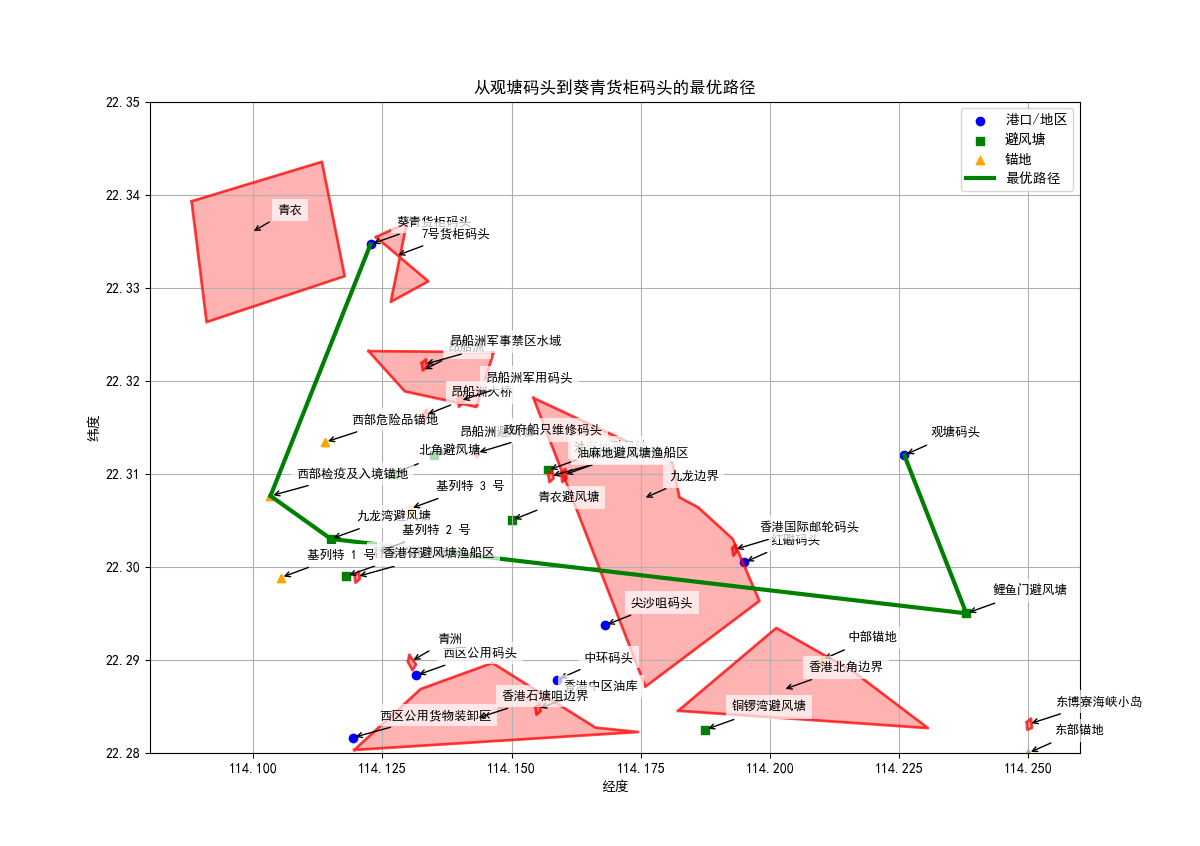
\includegraphics[width=0.8\textwidth]{Image/MD-Astar_BestPath.png}
    \captionof{figure}{5 从观塘码头到葵青货柜码头的最优路径(论文图4.3)}
\end{center}
\end{frame}

% 第5页:启发式函数可视化
\begin{frame}[plain]{启发式函数可视化展示}
\begin{center}
    \includegraphics[width=0.8\textwidth]{Image/MD-Astar_Heuristic.png}
    \captionof{figure}{6 启发式函数权重分布可视化(论文图4.1)}
\end{center}
\end{frame}

% 第6页:AN-MPC 控制器轨迹仿真实验
\begin{frame}{AN-MPC控制器轨迹仿真}
\justifying
控制模块采用 AN-MPC 策略进行轨迹优化与扰动补偿。

\vspace{0.5em}
\textbf{实验设置:}
\begin{itemize}
    \item 引入水流扰动,方向与速度随机扰动;
    \item 采用参考路径点进行滚动优化控制;
    \item 实验中提前 128s 到达终点,成功触发终止机制。
\end{itemize}
\end{frame}

% 第7页:控制器实验轨迹图展示
\begin{frame}[plain]{AN-MPC轨迹仿真图示}
\begin{center}
    \includegraphics[height=0.7\textwidth]{Image/AN-MPC_Result.png}
    \captionof{figure}{7 含水流扰动条件下的 MPC 路径跟踪结果(论文图4.4)}
\end{center}
\end{frame}
